\begin{frame}{Phases of water}
\centering
\only<1>{
\begin{tabular}{>{\centering\arraybackslash}p{.45\textwidth}>{\centering\arraybackslash}p{.45\textwidth}}
    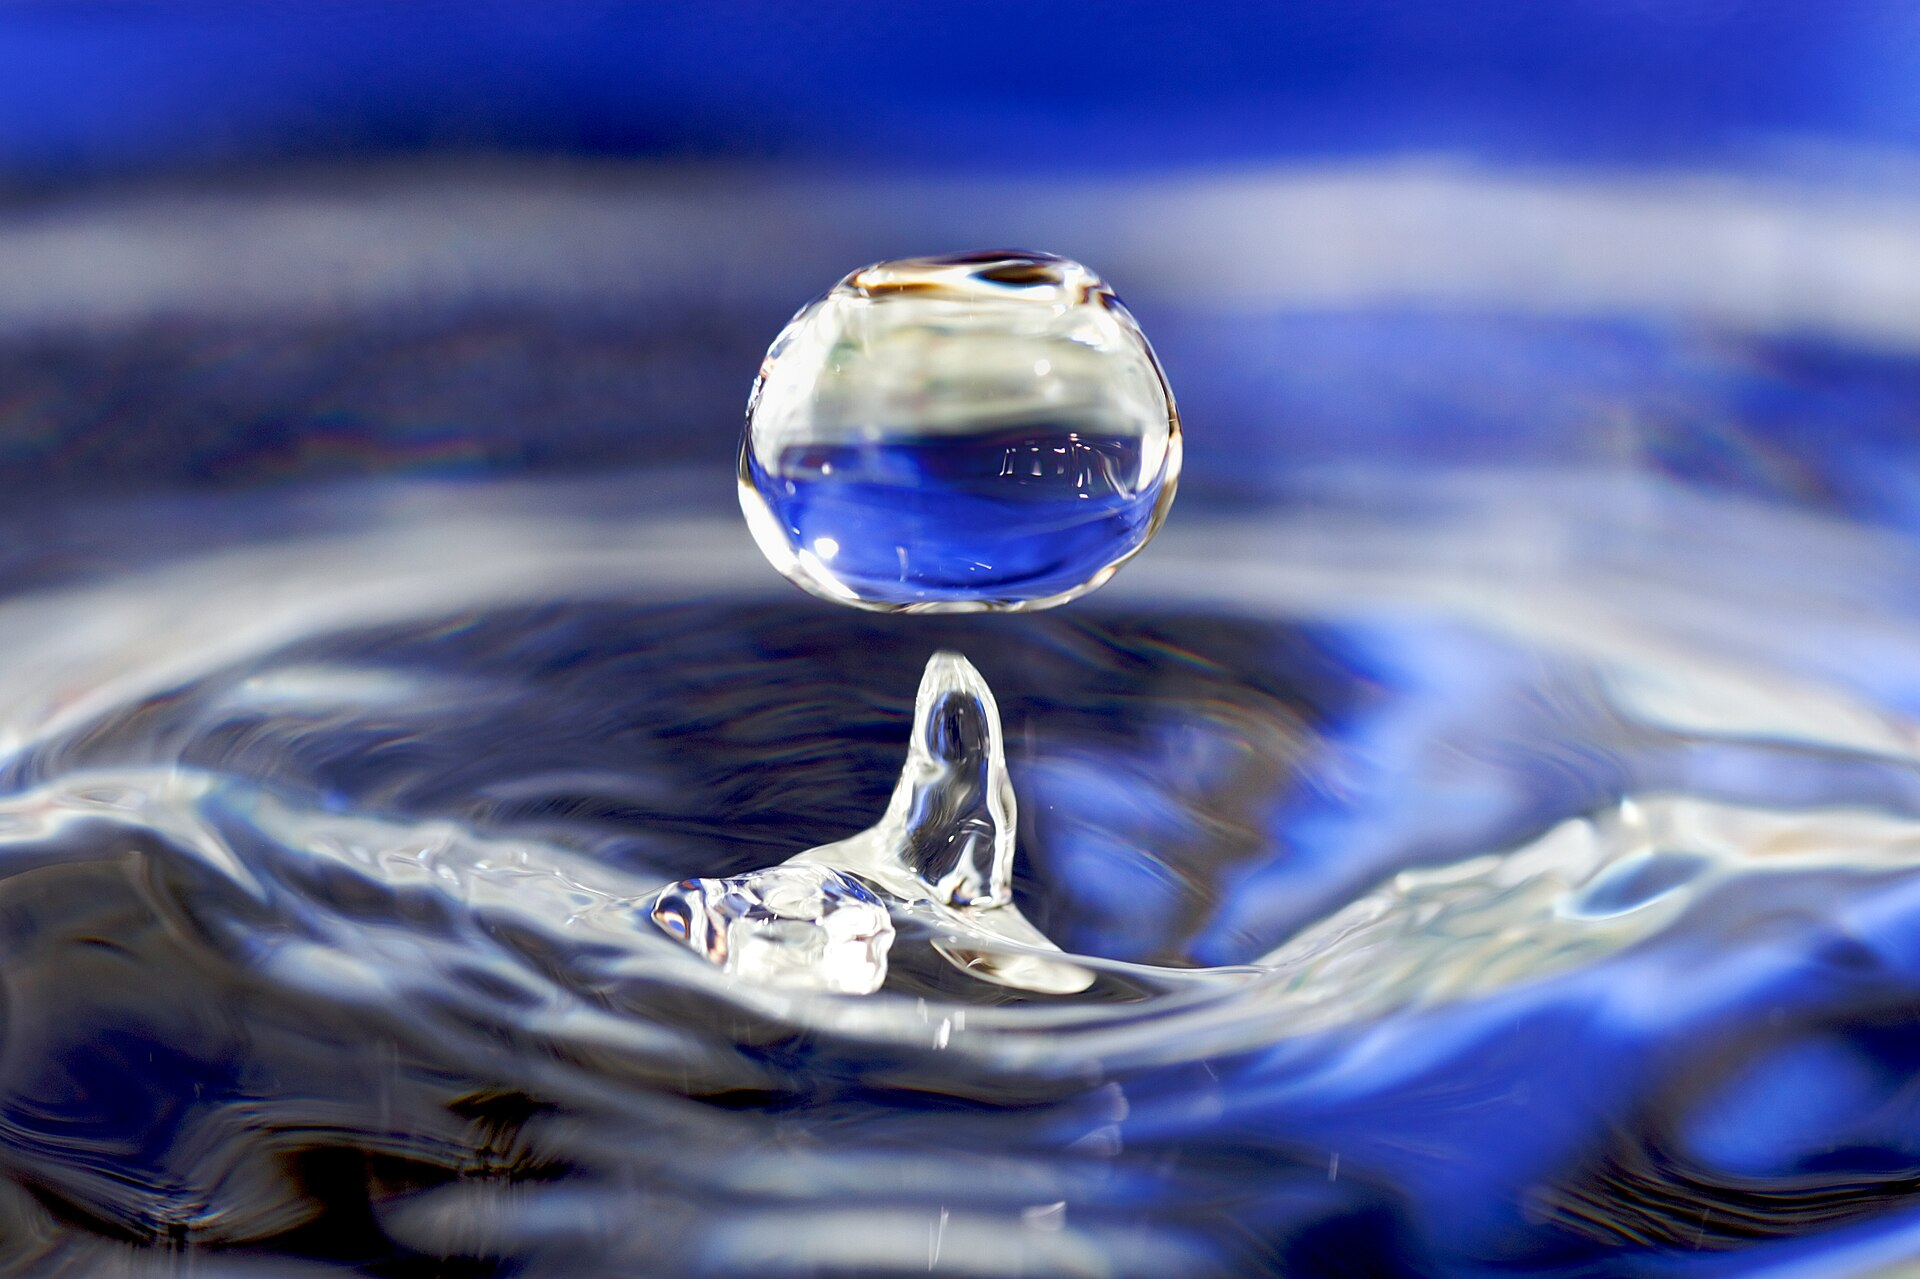
\includegraphics[width=.7\linewidth]{figs/water.jpg} & 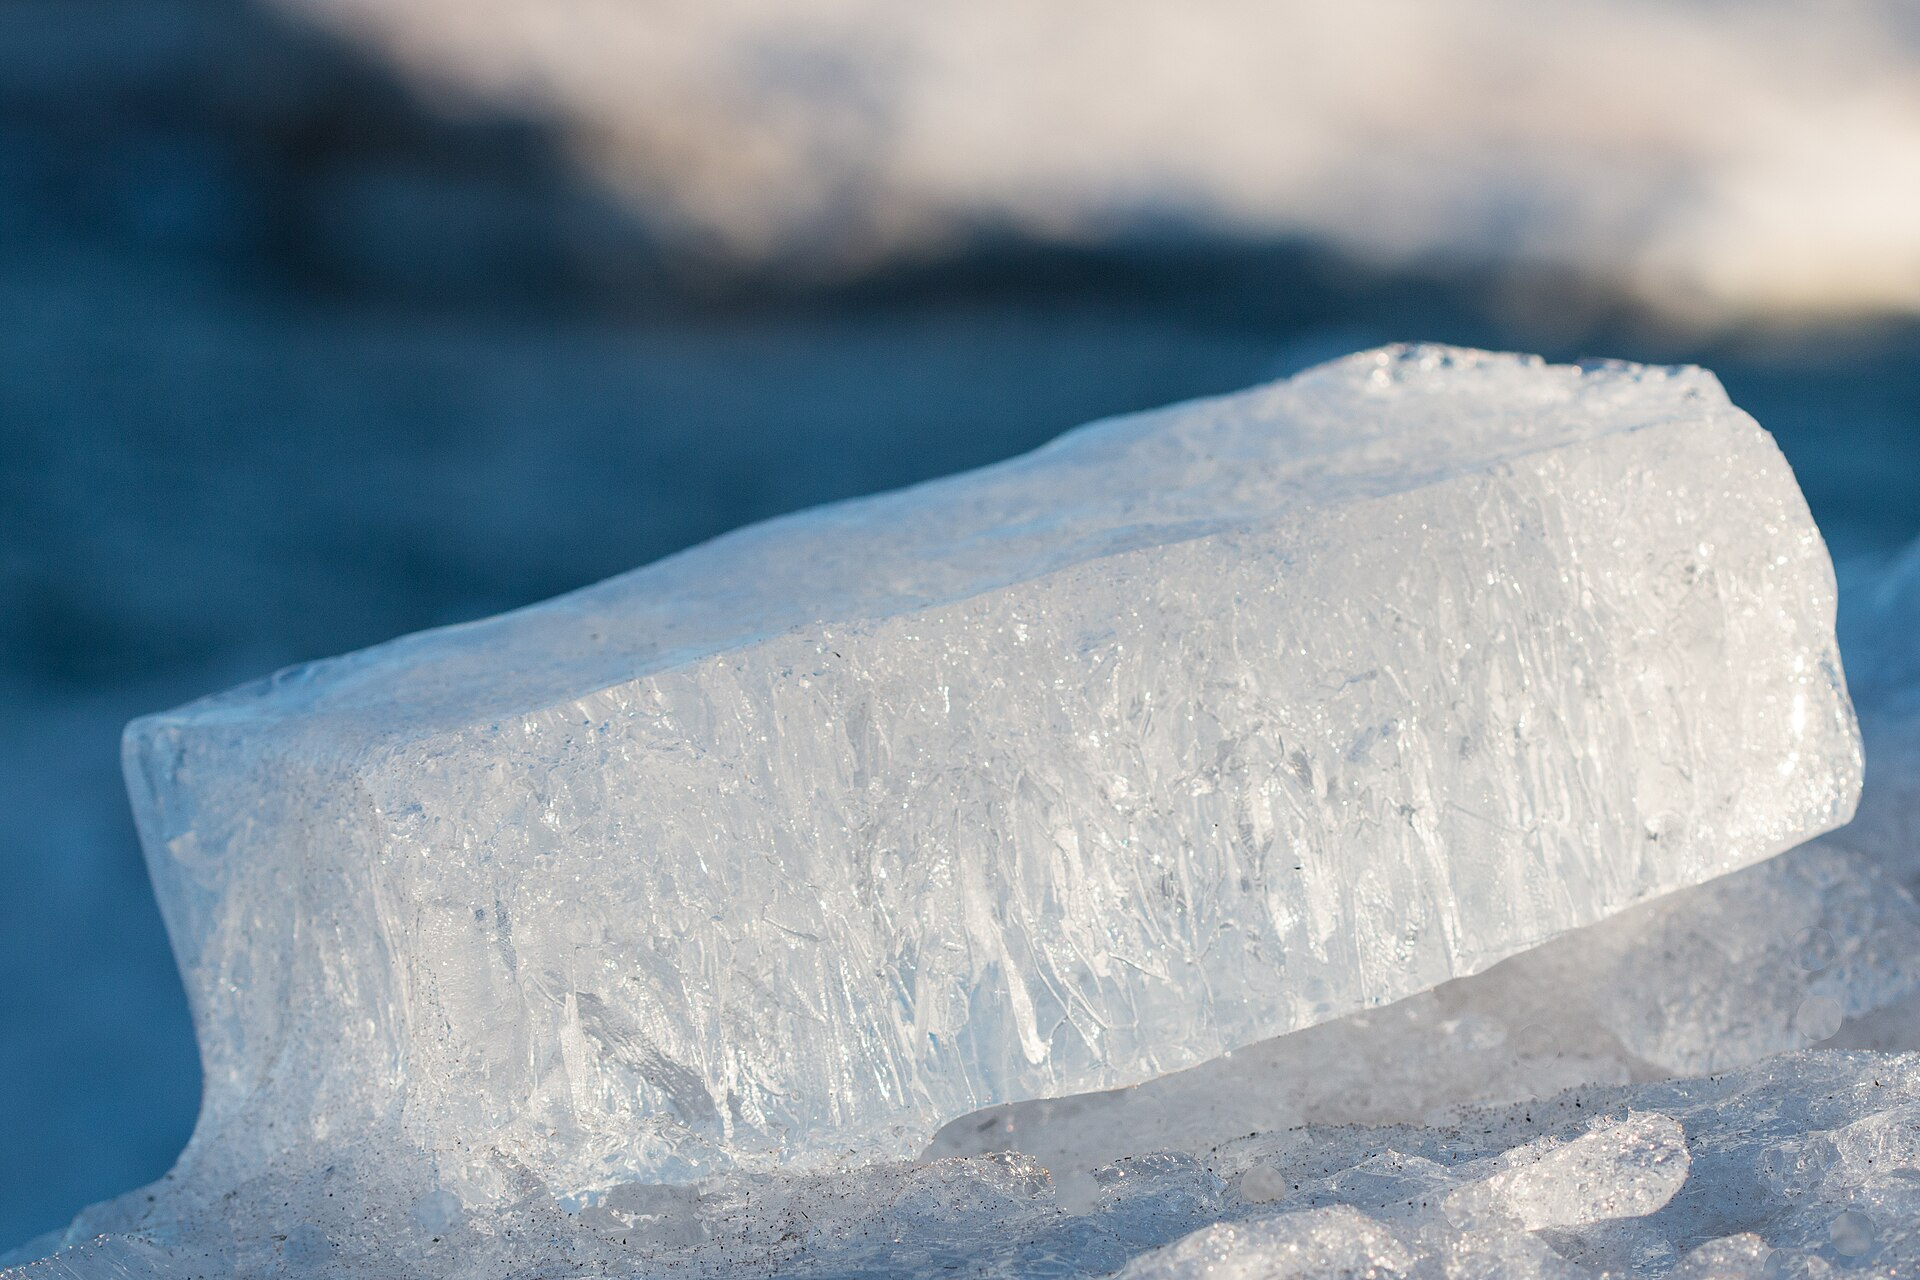
\includegraphics[width=.7\linewidth]{figs/ice.jpg}
\end{tabular}
}
\only<2>{
\begin{tabular}{>{\centering\arraybackslash}p{.45\textwidth}>{\centering\arraybackslash}p{.45\textwidth}}
    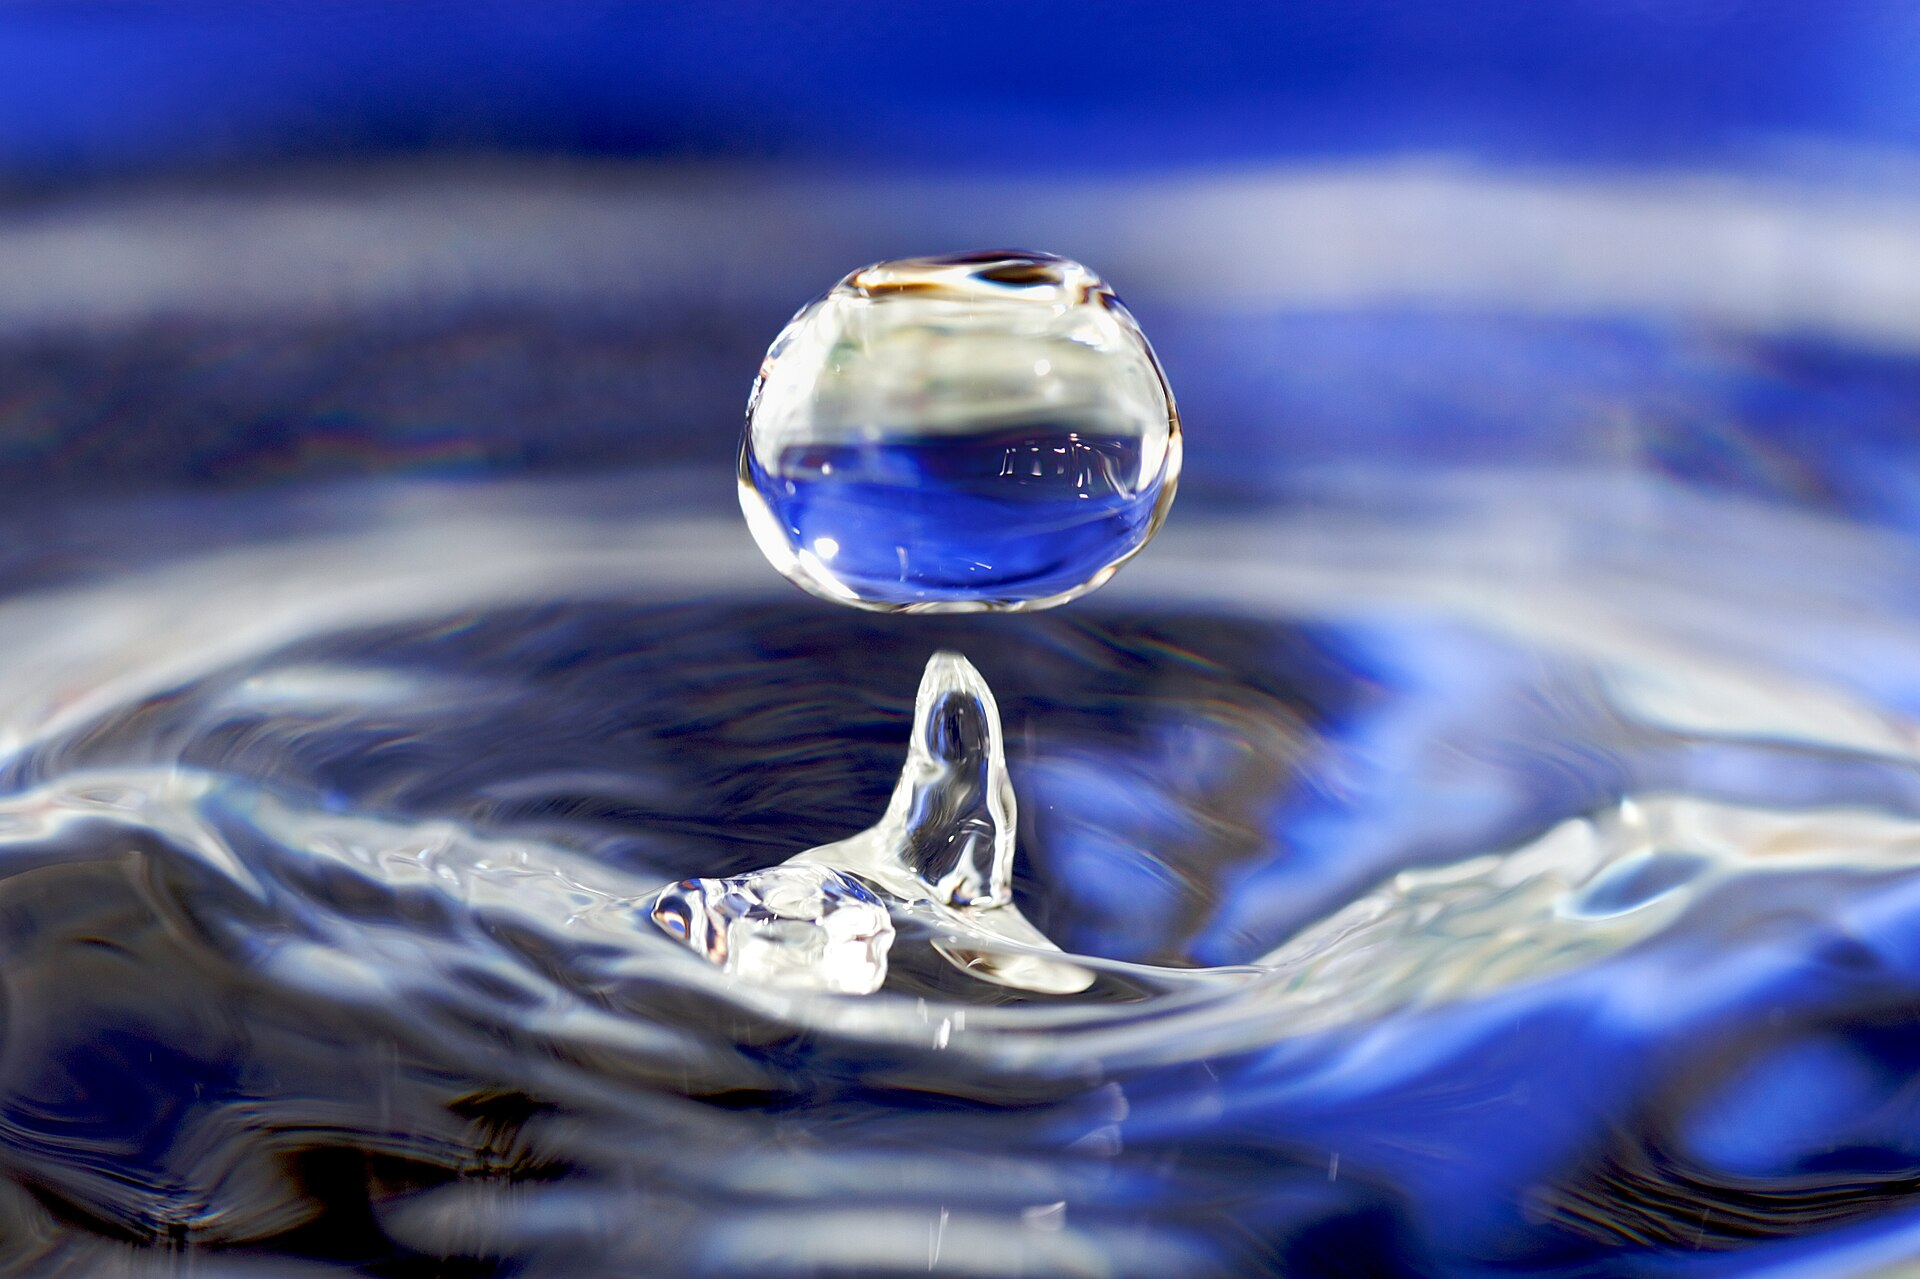
\includegraphics[width=.7\linewidth]{figs/water.jpg} & 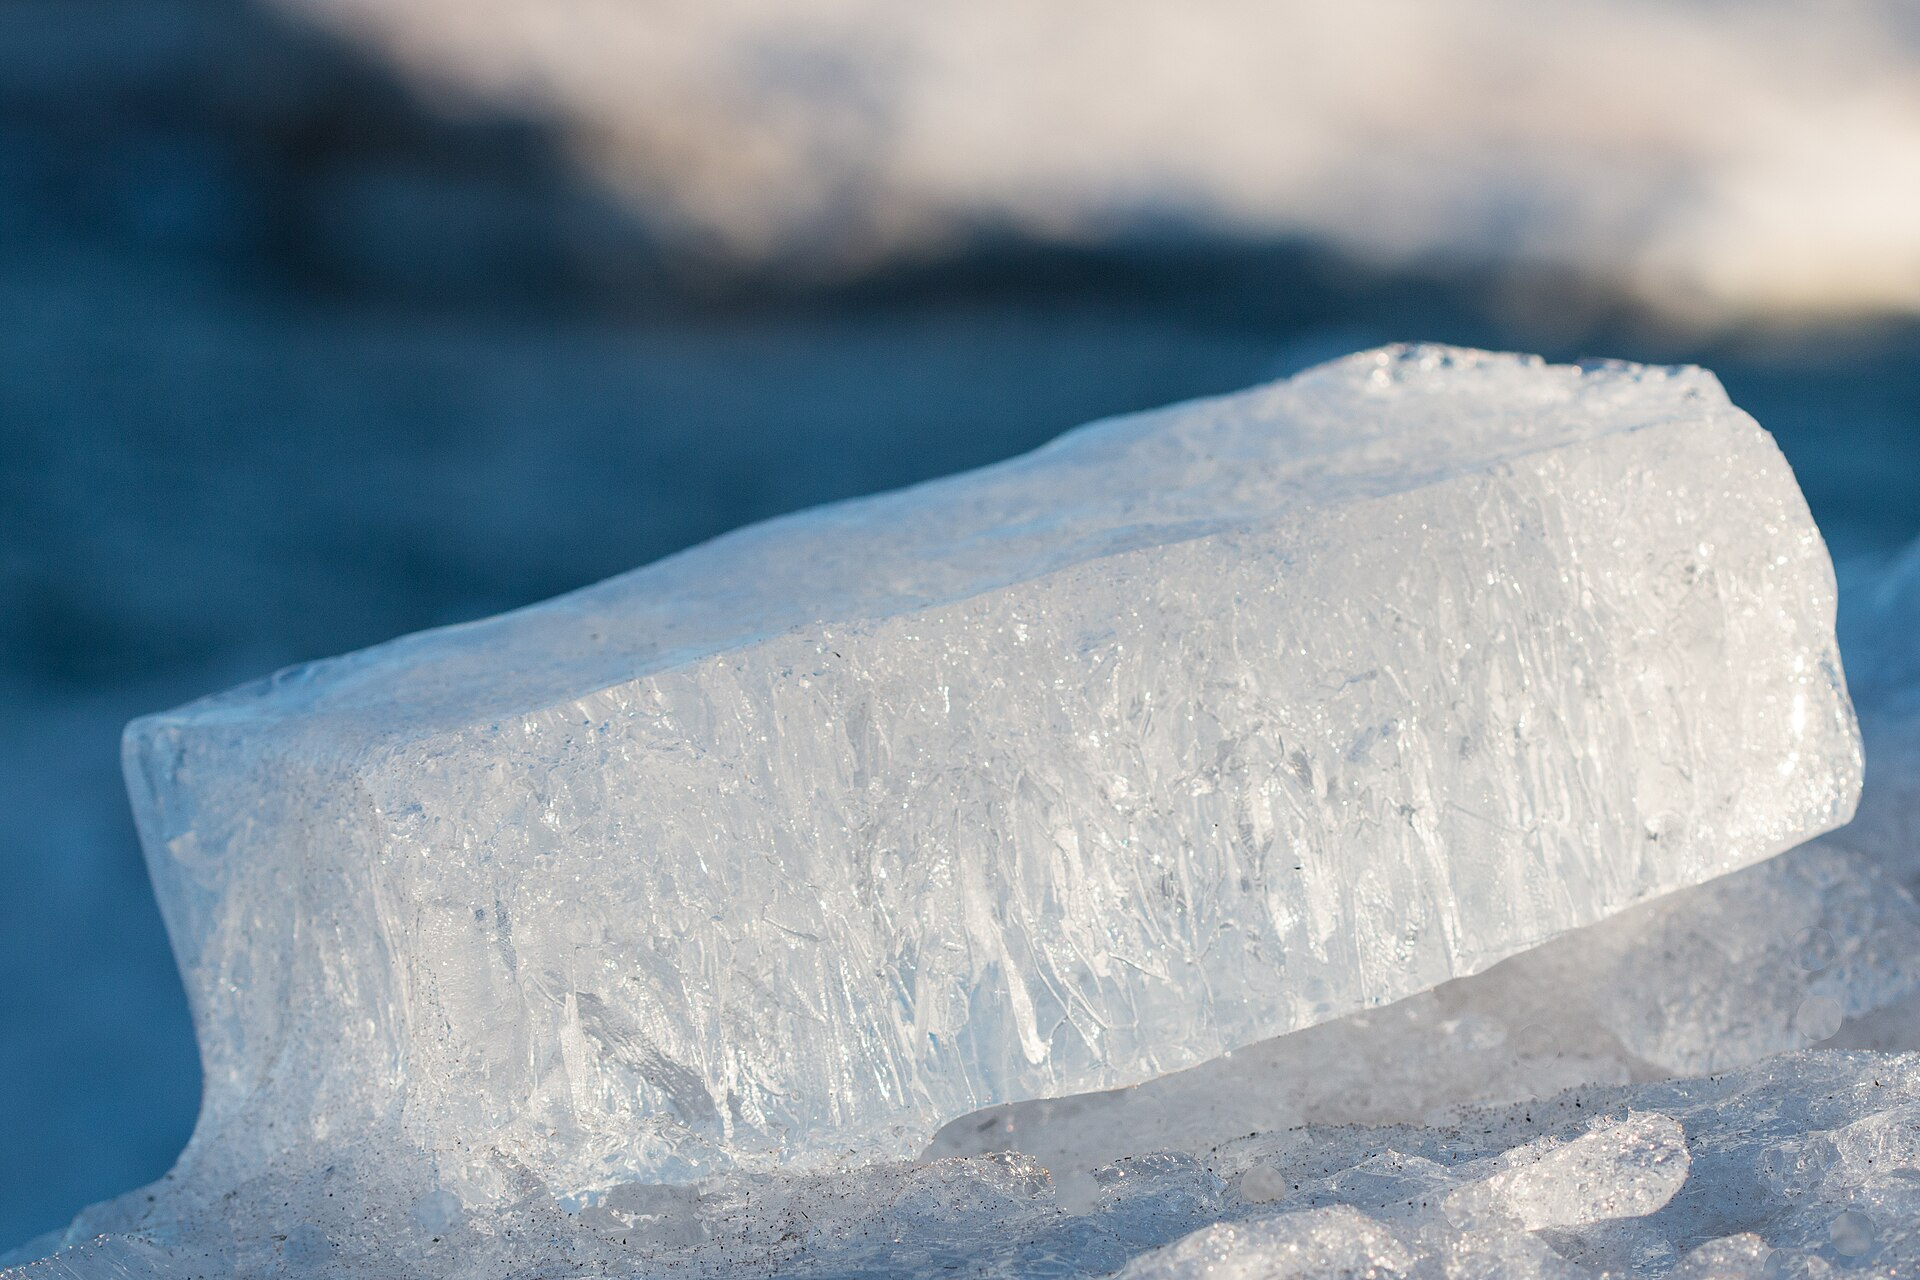
\includegraphics[width=.7\linewidth]{figs/ice.jpg} \\
    \addlinespace[1.5em]
    \Water & \IceLattice{1}
\end{tabular}
}
\end{frame}

\begin{frame}{Crystallography}
\centering
\begin{tabular}{>{\centering\arraybackslash}p{.45\textwidth}>{\centering\arraybackslash}p{.45\textwidth}}
    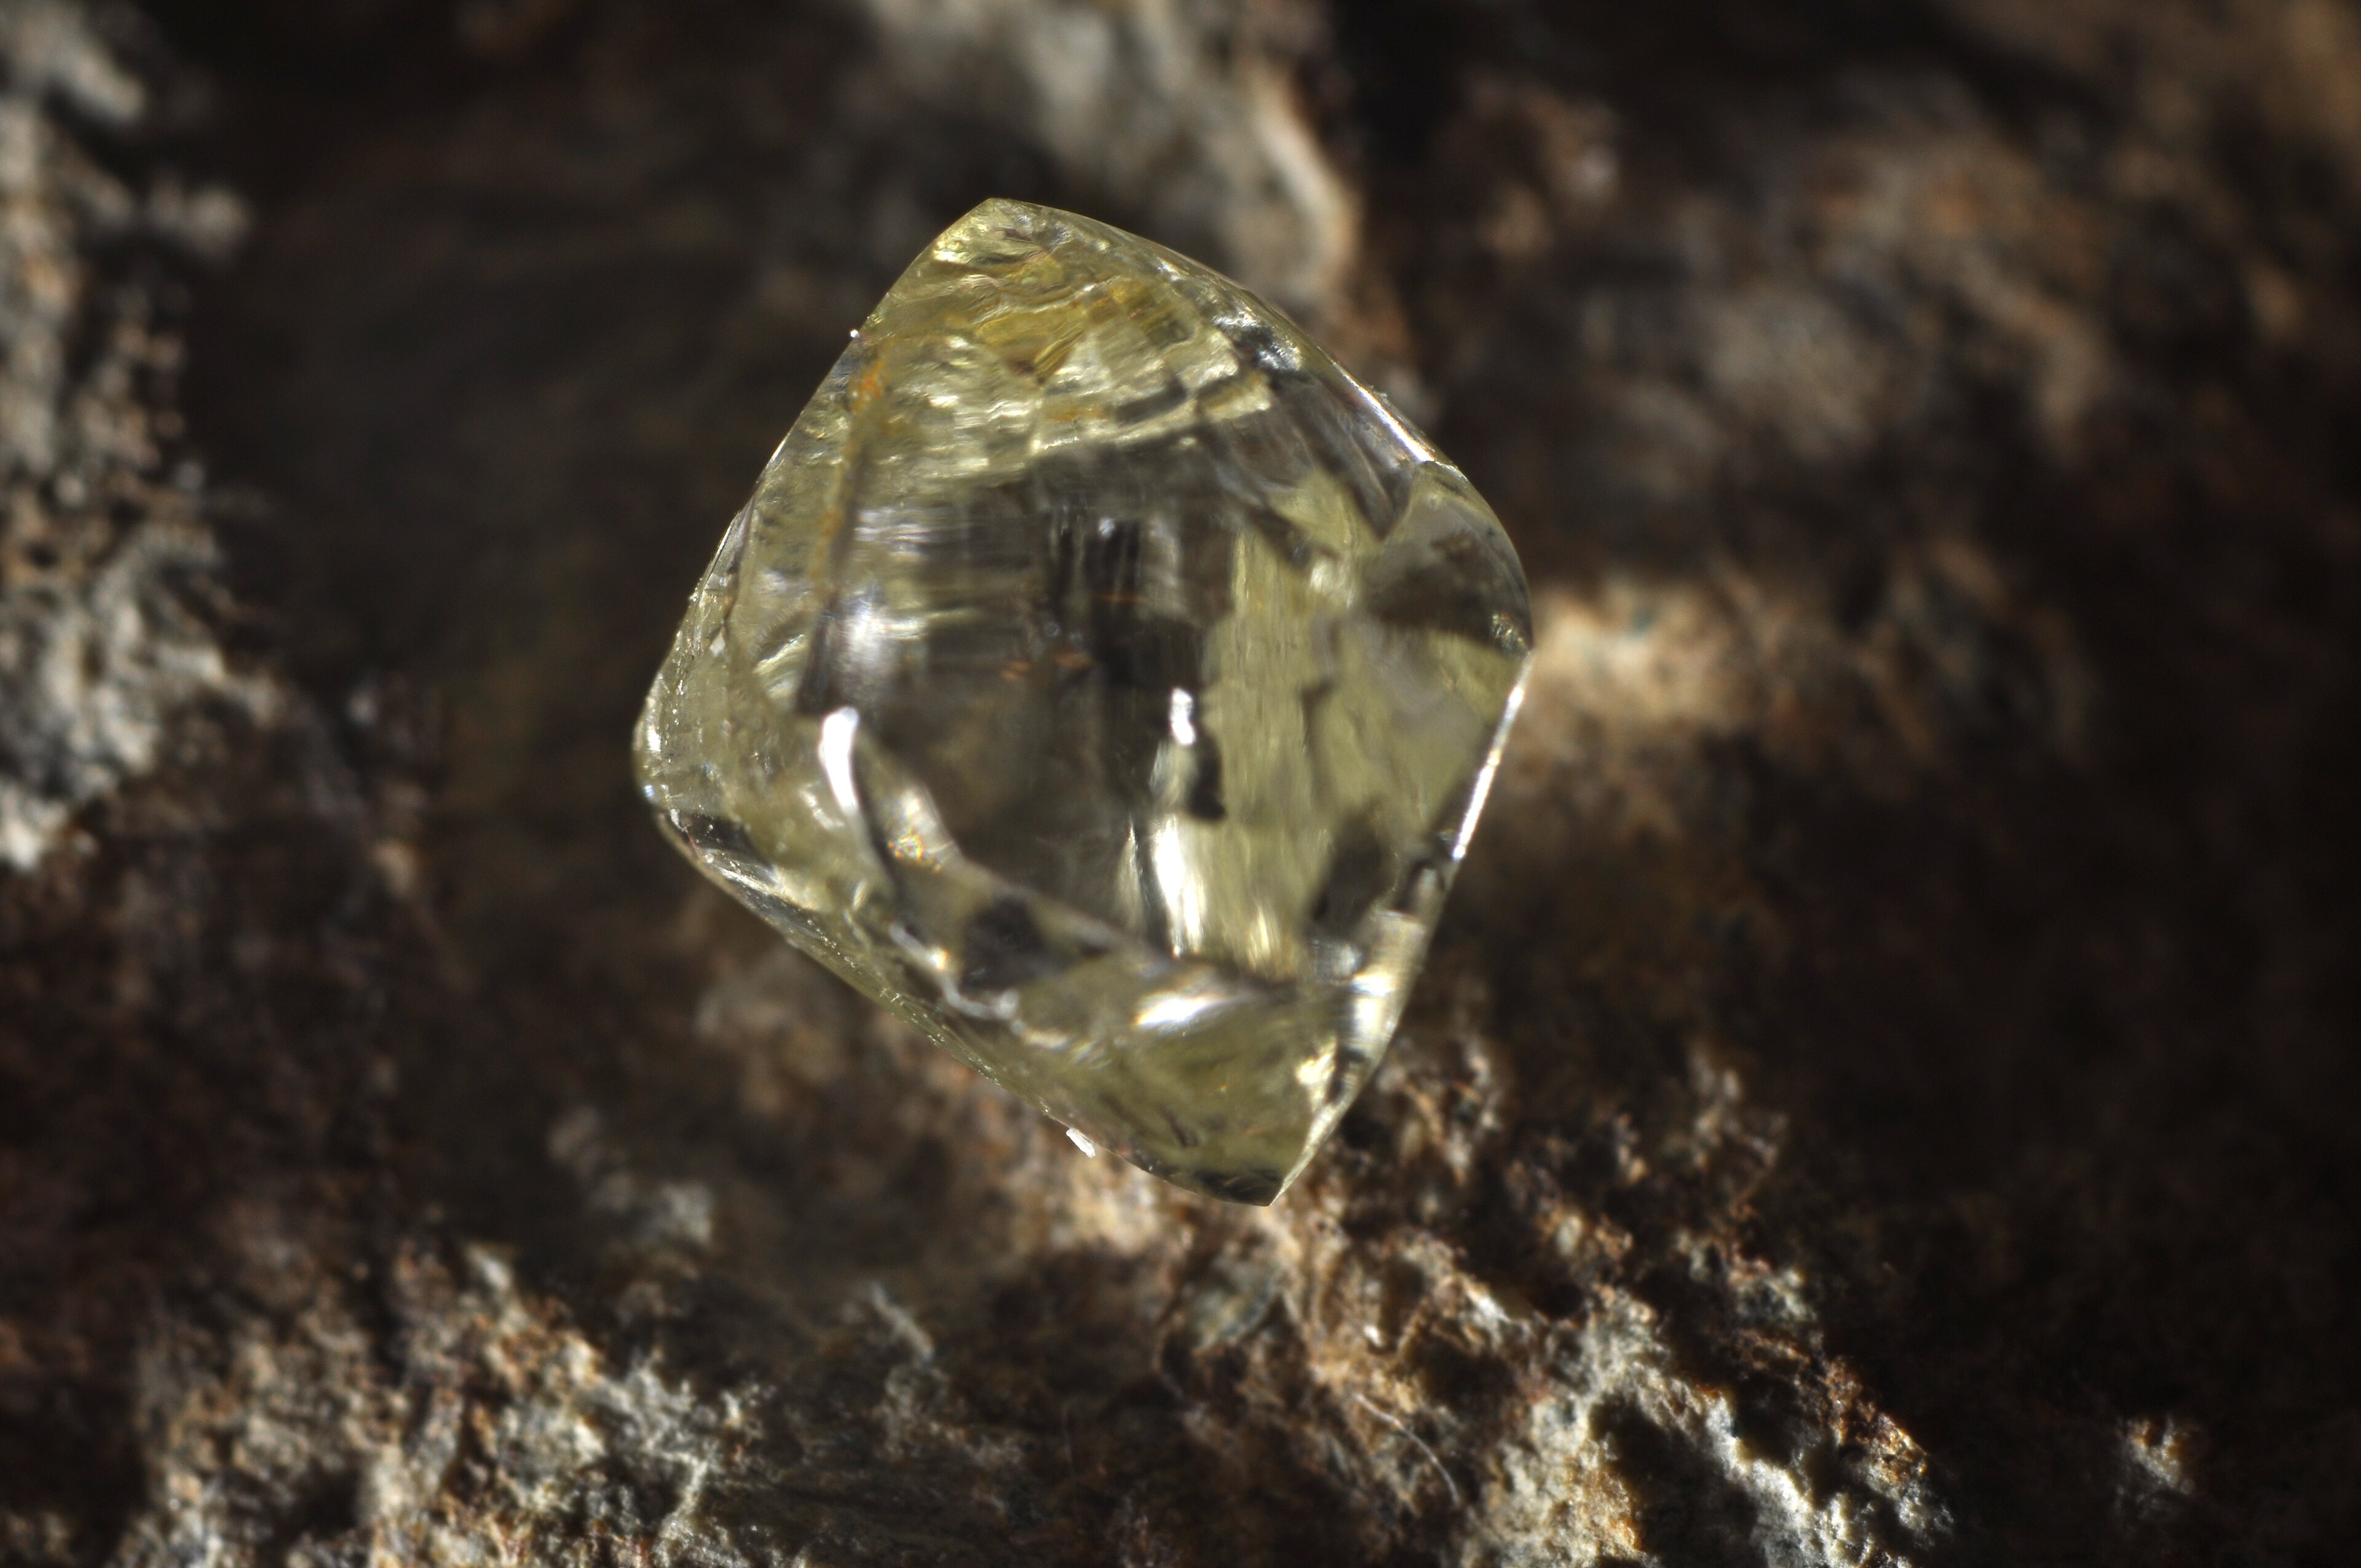
\includegraphics[trim={7cm 5cm 7cm 5cm},clip, width=.7\linewidth]{figs/Diamond.jpg} &
	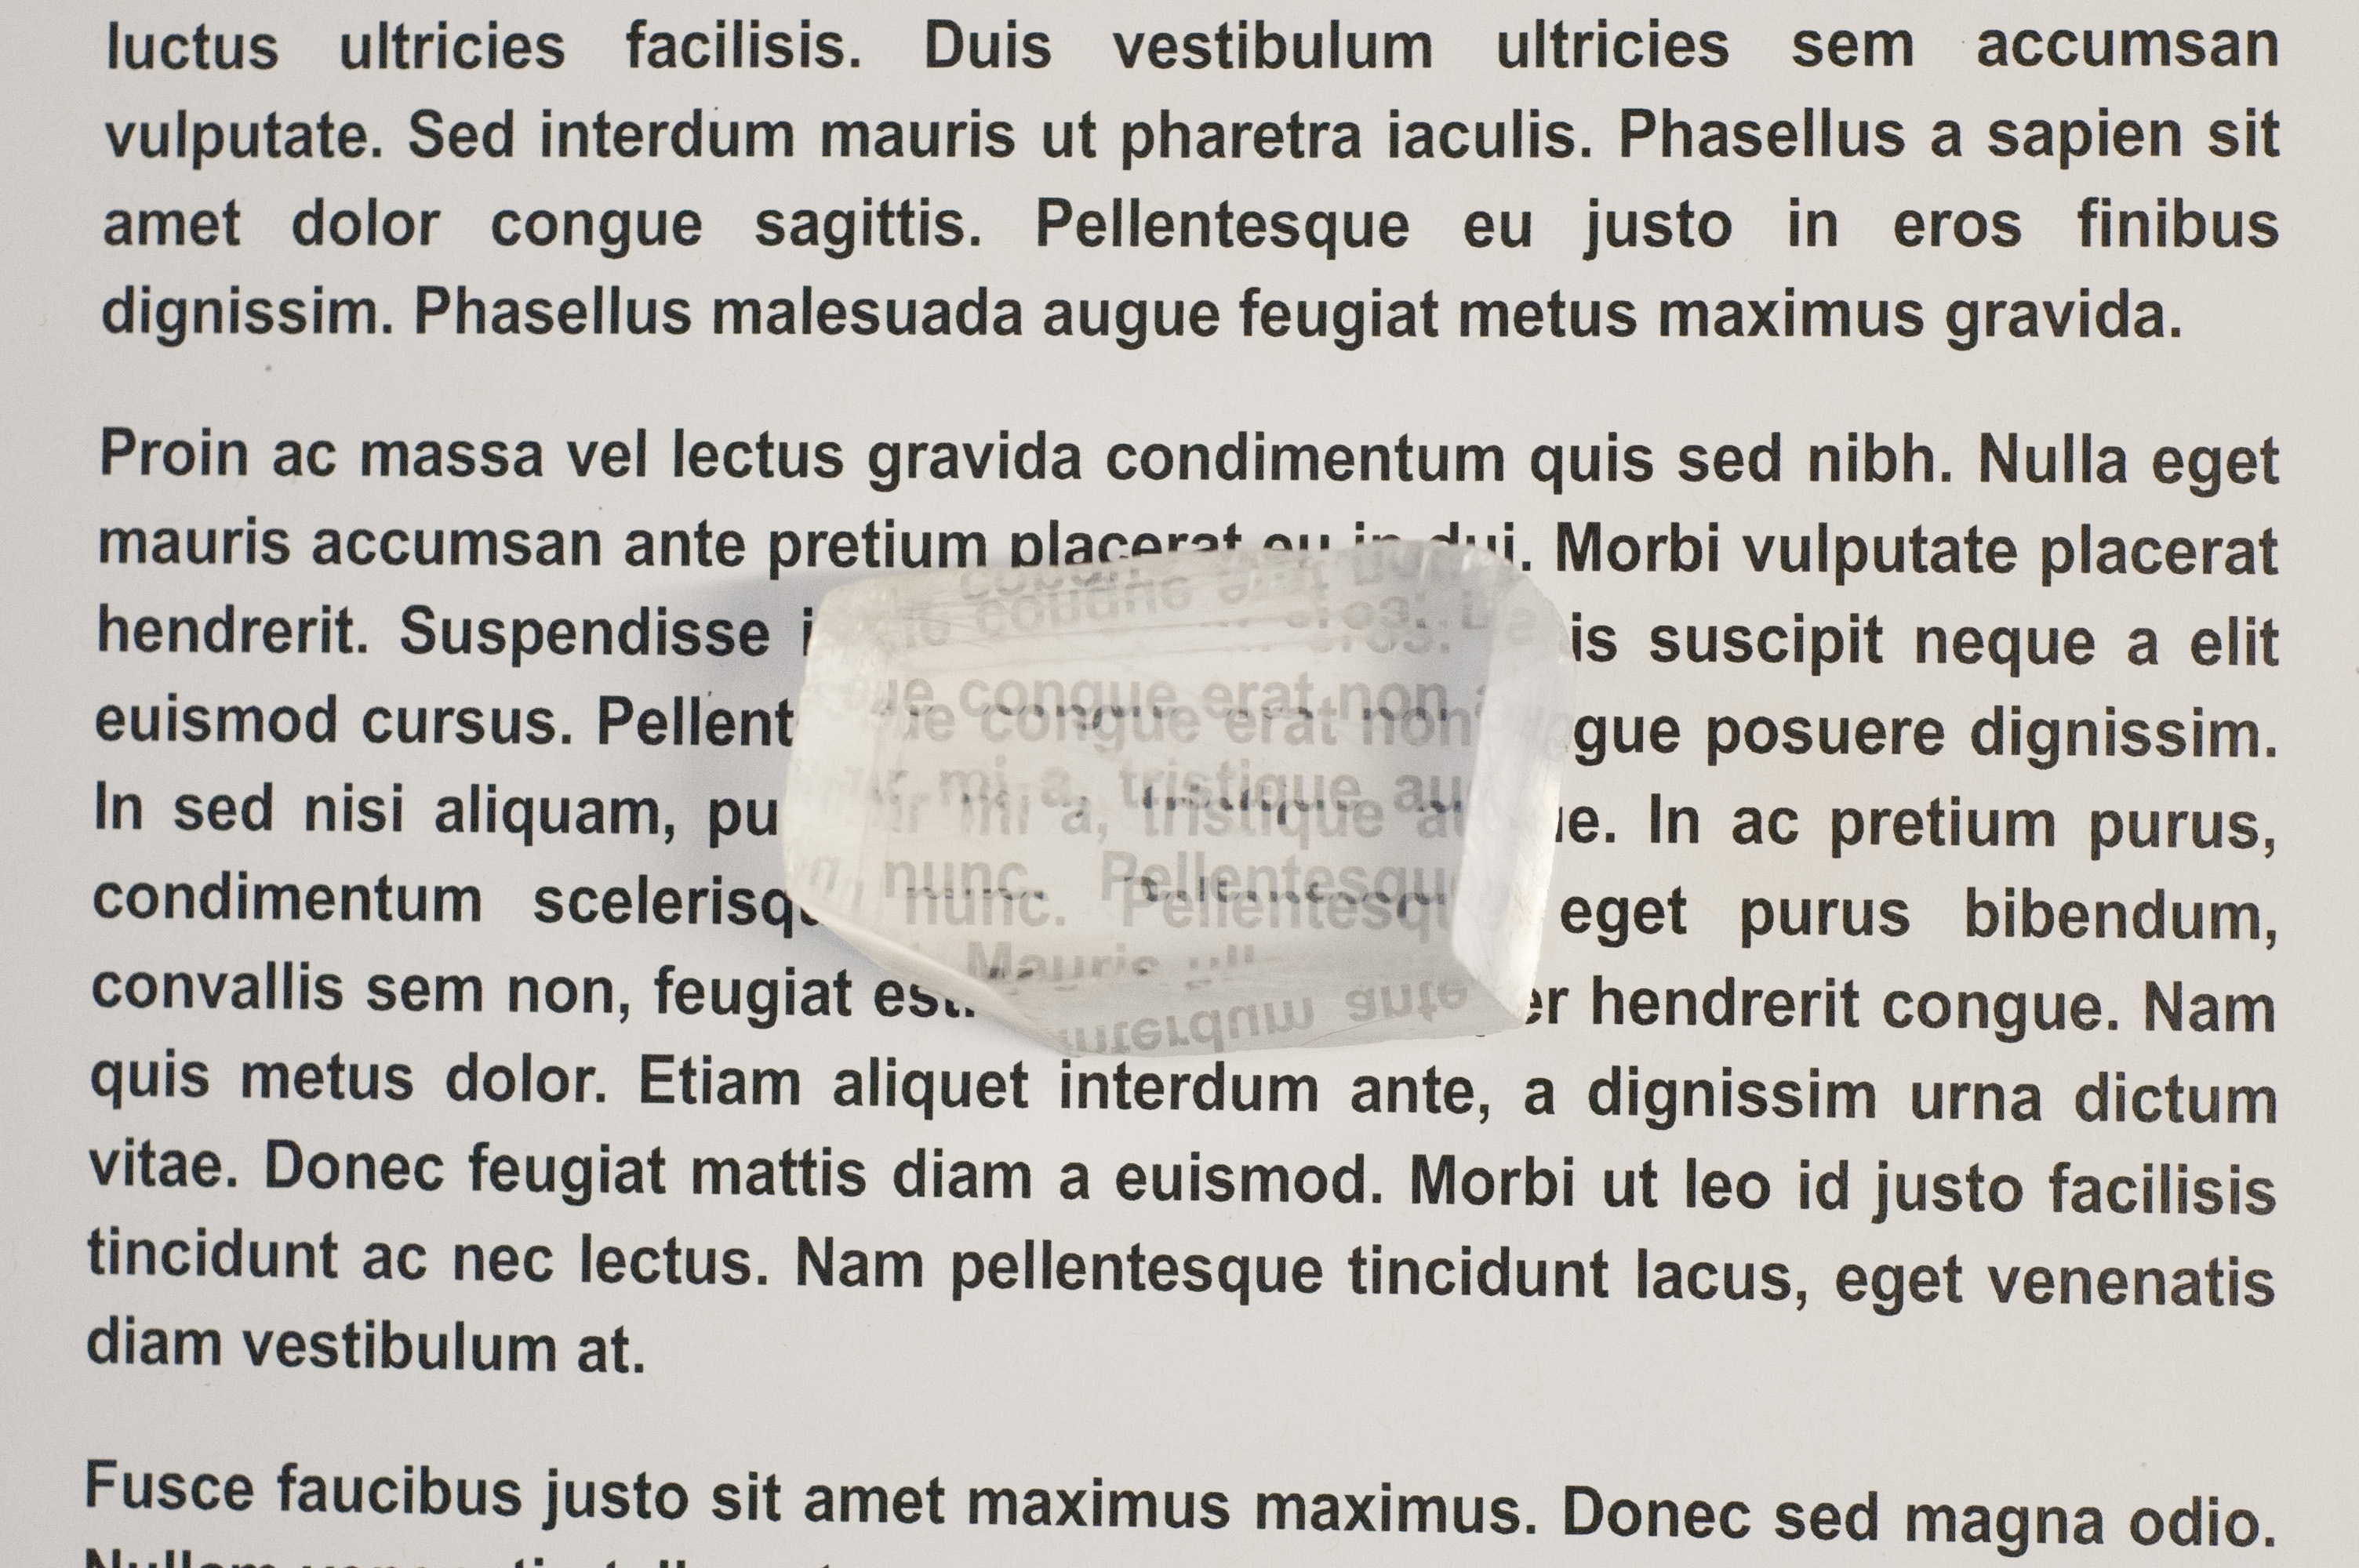
\includegraphics[trim={7cm 5cm 7cm 5cm},clip, width=.7\linewidth]{figs/Calcite.jpg} \\
    \addlinespace[2em]
	\DiamondUnitCell & \CalciteUnitCell 
\end{tabular}

\medskip

The \emph{ordering} of the atoms determines the macroscopic properties
\end{frame}

\begin{frame}{Symmetry}
\centering
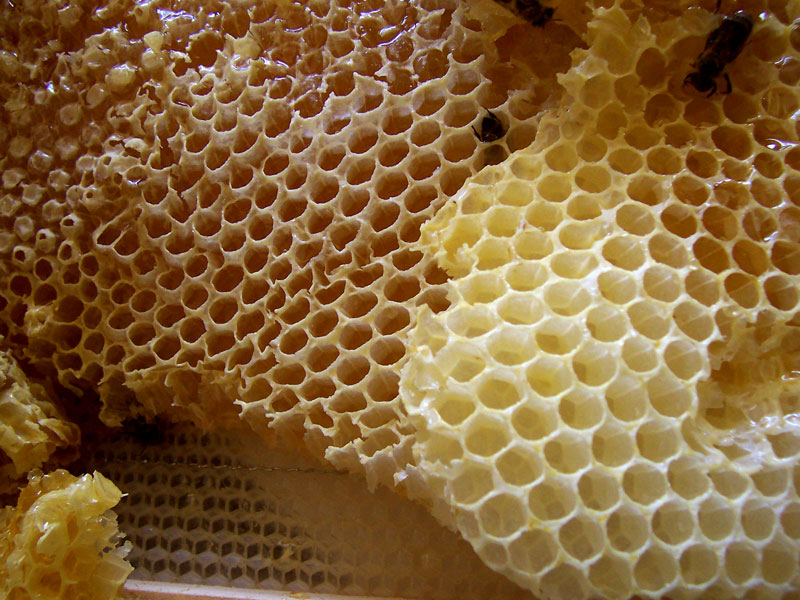
\includegraphics[height=2.6cm]{figs/Honeycomb.jpg}\qquad
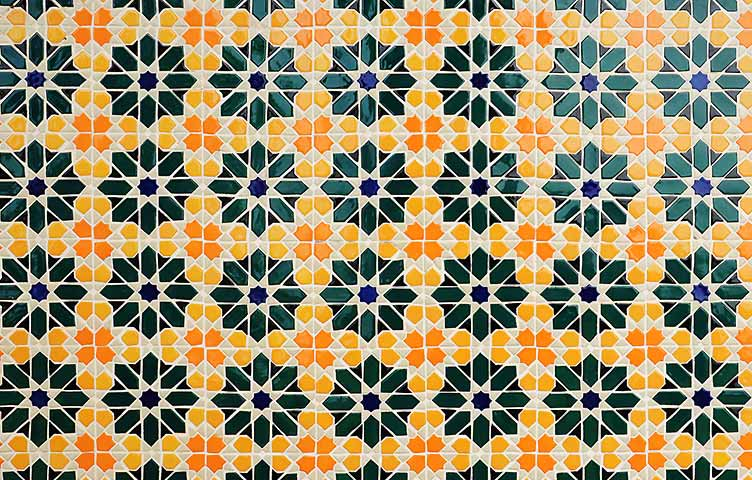
\includegraphics[height=2.6cm]{figs/Mosaic.jpg}

\bigskip

\MexicanHat

\bigskip
Symmetry $=$ transformations that leave structure invariant
\end{frame}

\begin{frame}{Order breaks symmetry}
\centering
\begin{tabular}{>{\centering\arraybackslash}p{.45\textwidth}>{\centering\arraybackslash}p{.45\textwidth}}
	\Water & \IceLattice{1} \\
	\addlinespace[1em]
	Water: continuous shifts and rotations & Ice: lattice translations and rotations
\end{tabular}

\bigskip
\uncover<2->{More order $=$ less symmetry}
\end{frame}

\begin{frame}{Curie \& Landau}
\begin{columns}[T]
\column{.48\textwidth}
\centering
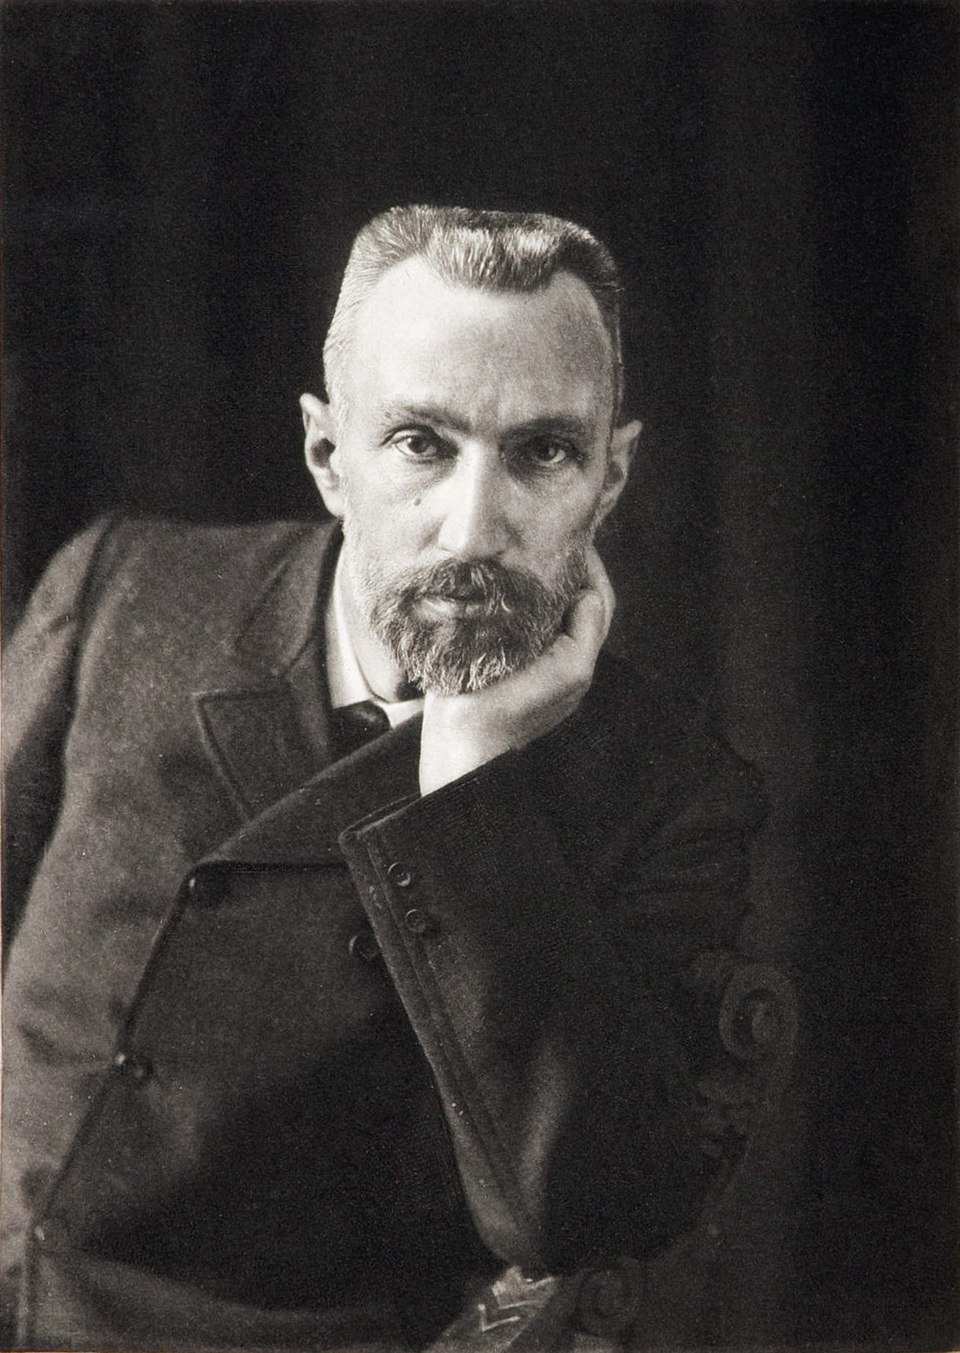
\includegraphics[height=2.8cm]{figs/Curie.jpg}

\medskip
{\it C'est la dissymétrie qui crée le phénomène.}

\smallskip
{\small It is dissymmetry that creates the phenomenon.}

\smallskip
{\scriptsize P.~Curie (1894)}
\column{.48\textwidth}
\centering
\uncover<2->{%
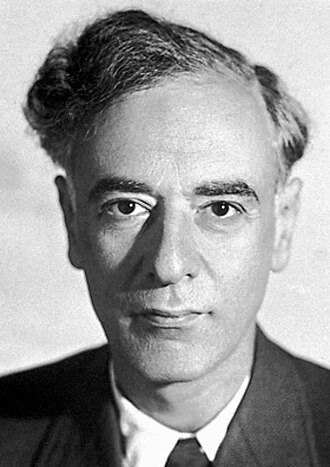
\includegraphics[height=2.8cm]{figs/Landau.jpg}

\medskip
{\it But elements of symmetry are either present or absent; no intermediate case is possible.}

\smallskip
{\scriptsize L.~Landau (1937)}}
\end{columns}

\bigskip
\centering
\uncover<3->{Even if the underlying physics is symmetric, phenomena often break this.}
\end{frame}

\begin{frame}{Ferromagnets}
\begin{columns}[c]
\column{.38\textwidth}
\centering
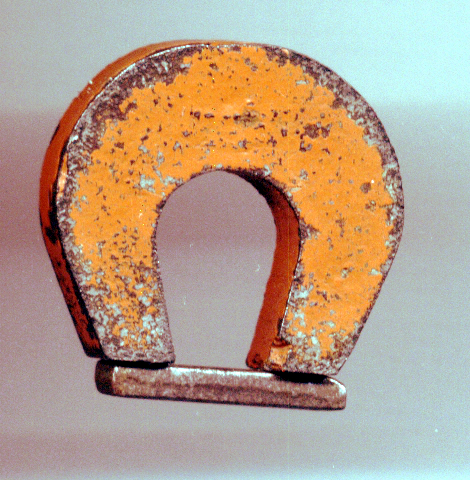
\includegraphics[height=3cm]{figs/Magnet}
\column{.6\textwidth}
\centering
\uncover<2->{\FerroFade{1}}
\end{columns}

\bigskip
\begin{columns}[c]
\column{.38\textwidth}
\centering
\uncover<3->{Could a magnet be made of many tiny magnets?}

\medskip
\uncover<6->{But what \emph{is} one tiny magnet?}
\column{.6\textwidth}
\centering
\uncover<4->{%
	\only<-4>{\MagneticOrder{1}}%
	\only<5->{\MagneticOrder{2}}}
\end{columns}
\end{frame}